\section{Séquencement}
	\label{sec:sequencement}

	\subsection{Diagramme de Gantt}
		Le très très beau diagramme de Gantt est visible \ffigure{} \ref{fig:gantt}. Sinon on a environ rien à dire à son propos.

	\subsection{Planning des charges}
		Un truc qui ressemble à un planning des charges est visible \ffigure{} \ref{fig:planning_charge}.

		\begin{landscape}
		 	\begin{figure}
	            \centering
	            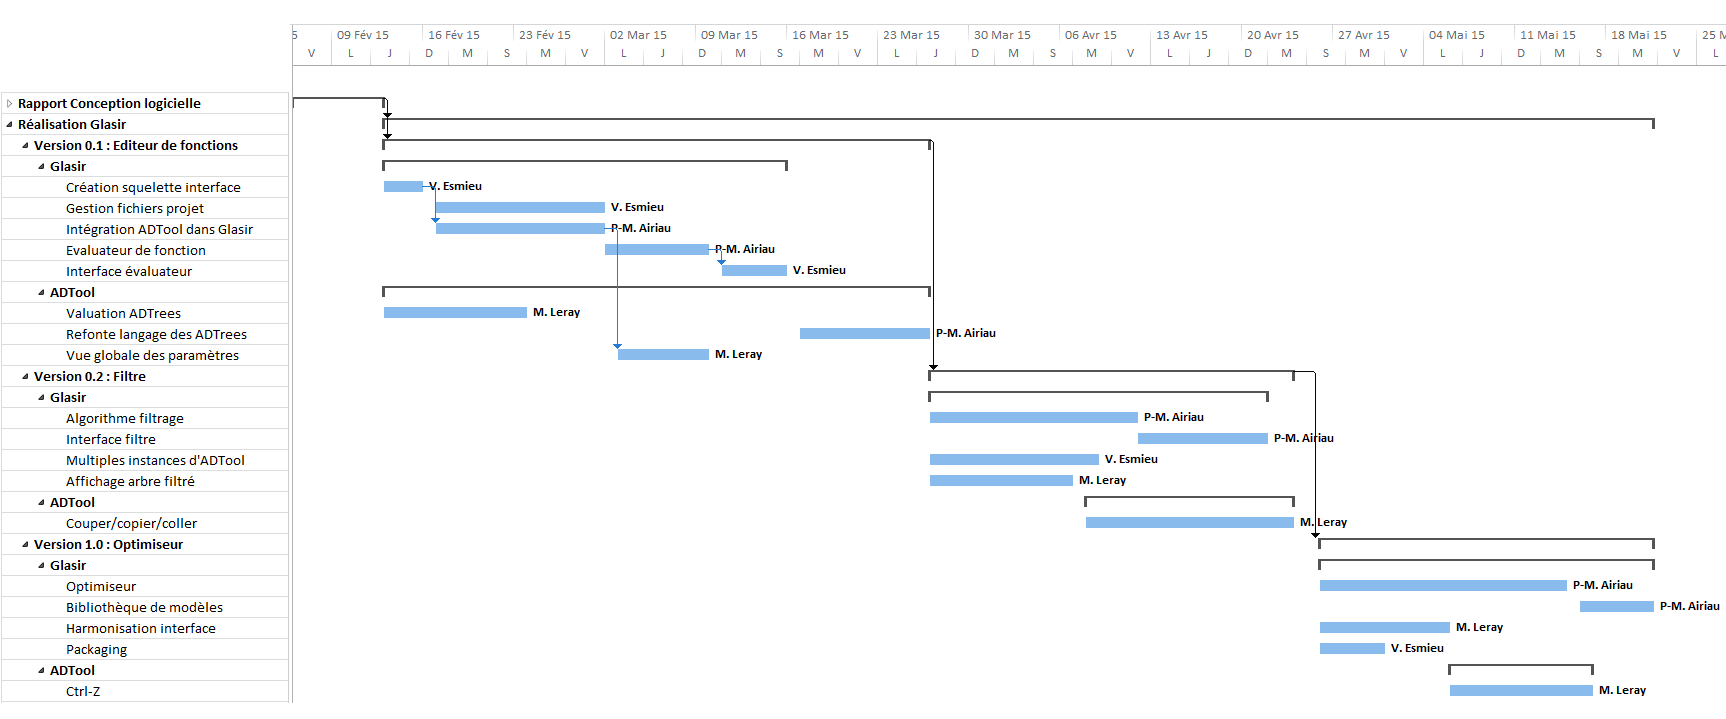
\includegraphics[height=0.70\textwidth]{figure/DiagGantt.png}
	            \caption{Diagramme de Gantt présentant la chronologie des tâches.}
	            \label{fig:gantt}
	        \end{figure}
	    \end{landscape}

		\begin{landscape}
		 	\begin{figure}
	            \centering
	            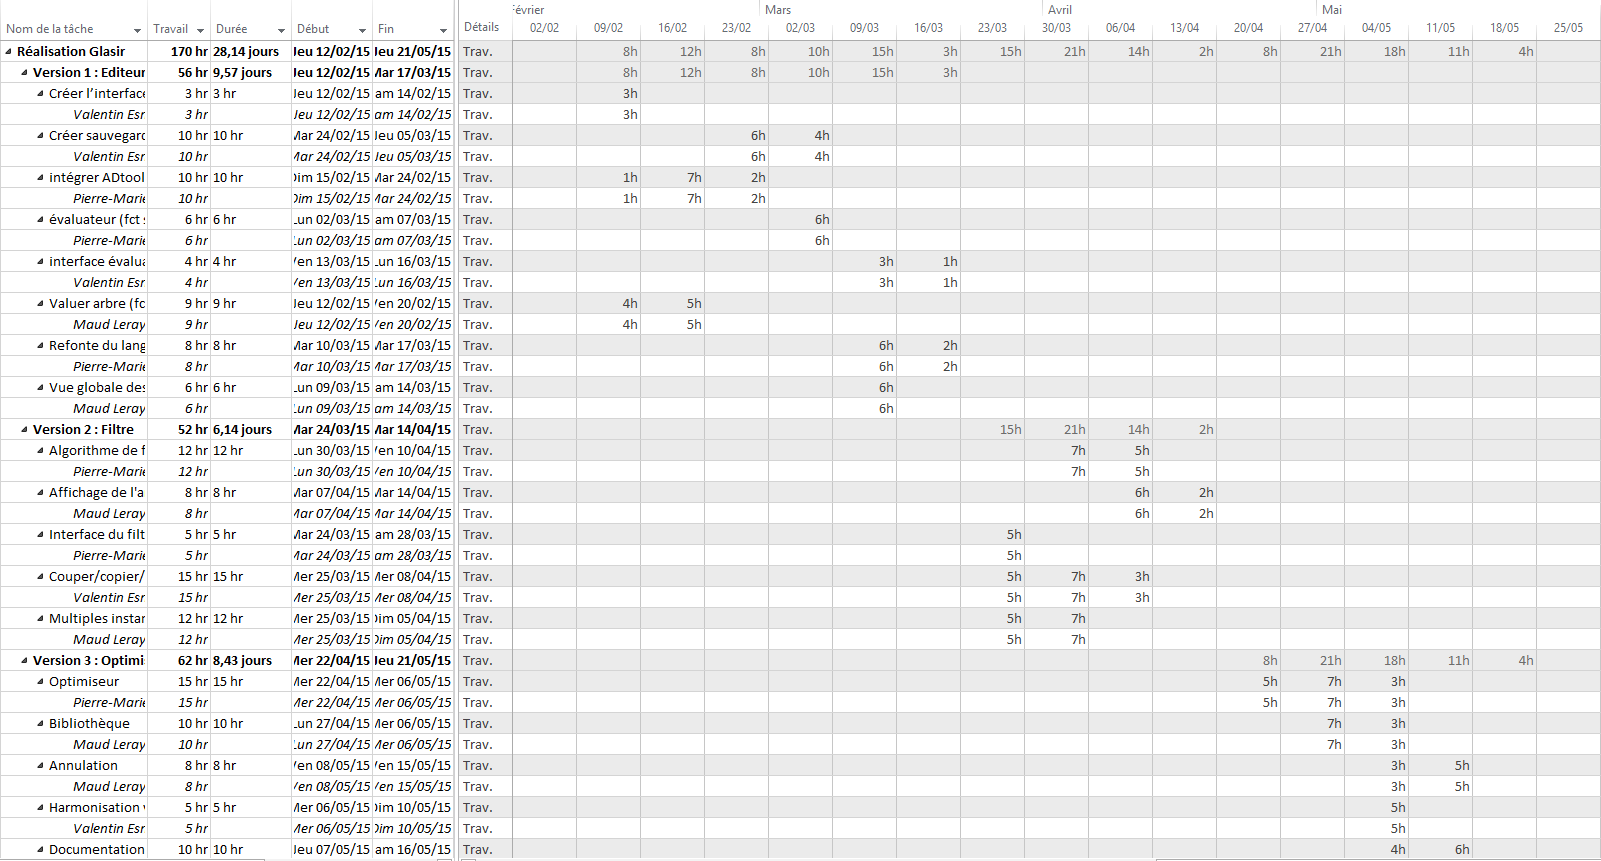
\includegraphics[height=0.70\textwidth]{figure/RepartitionTaches2.png}
	            \caption{Planning des charges super cheum}
	            \label{fig:planning_charge}
	        \end{figure}
	    \end{landscape}